\documentclass[12pt]{article}
\input{/Users/circle/Documents/博一下/homework/setting.tex}
\setcounter{secnumdepth}{2}
\usepackage{autobreak}
\usepackage{amsmath}
\setlength{\parindent}{2em}
\graphicspath{{../}}
\ziju{0.1pt}

%pdf文件设置
\hypersetup{
	pdfauthor={袁磊祺},
	pdftitle={高等实验流体力学小作业}
}

\title{
		\vspace{-1in} 	
		\usefont{OT1}{bch}{b}{n}
		\normalfont \normalsize \textsc{\LARGE Peking University}\\[0.2cm] % Name of your university/college \\ [25pt]
		\horrule{0.5pt} \\[0.2cm]
		\huge \bfseries{高等实验流体力学小作业} \\[-0.2cm]
		\horrule{2pt} \\[0.2cm]
}
\author{
		\normalfont 								\normalsize
		College of Engineering \quad 2001111690  \quad 袁磊祺\\	\normalsize
        \today
}
\date{}

\begin{document}

\input{/Users/circle/Documents/博一下/homework/setc.tex}

\maketitle

\section{1}

\begin{itemize}
	\item 阅读误差分析方法中,关于数据拟合的相关知识,重点以线性拟 合为主。
	\item 分析随机误差对拟合结果的影响。
\end{itemize}

自 1794 年高斯提出按最小二乘准则估计未知参数以来,测量平差中一直采用最小二乘准则或最小二乘原理估计未知参数。它是测量中求未知参数估值最普遍、最主要的 方法,在其他科学领域中也有广泛的应用。

\subsection{最小二乘估计准则}

介平差问题一旦选定了数学模型,进行平差时,就要以这个模型为基础。由于测 量值含有误差,在有了多余观测值的情况下,即观测值的个数 $n$ 总是大于待估参数的个 数 $t$ 的情况下, 待估参数的解不定, 也就是观测值与选定的数学模型不相适应。平差的 任务就是想办法使观测值适应模型。为了使观测值适应数学模型,必须对观测值进行处
理,处理后的观测值称为估值,设原观测向量为 $\bm{L}$, 处理后的观测向量为 $\hat{\bm{L}}$, 两者之差
\begin{equation}
	\bm{V}=\hat{\bm{L}}-\bm{L}
\end{equation}
称为改正数或残差。

估值 $\hat{L}$ 满足数学模型,但要知道 $\hat{L}$ ,首先要求出 $V$, 使 $\hat{L}$ 满足数学模型的残差向量
$V$ 可能有很多。为了得到唯一的残差向量 $\bm{V}$, 就必须有一个准则,可用的准则很多,在
测量中通常用最小二乘准则,即
\begin{equation}
	\bm{V}^{\mathrm{T}} \bm{P} \bm{V}=\min
	\label{eq:11}
\end{equation}
式中, $\bm{P}$ 为权矩阵,它是适当选定的对称正定矩阵。

根据最小二乘准则,求观测向量的估值 $\hat{\bm{L}}$, 称为最小二乘平差。

\cref{eq:11}表明,在考虑权矩阵 $\bm{P}$ 的情况下,尽量使 $\hat{\bm{L}}$ 接近 $\bm{L}$ 或使残差向量 $\bm{V}$ 尽可 能地小。由此可见数学模型和观测向量 $\bm{L}$ 在平差中的重要性。数学模型是平差的基础, 对于给定的观测向量 $\bm{L}$, 按最小二乘准则进行平差,使平差值 $\hat{\bm{L}}$ 尽量接近 $\bm{L}$, 这就是平差问题的实质。

应当指出,上面给出的最小二乘准则并不需要观测向量 $\bm{L}$ 具有任何统计信息,而且 $\bm{P}$ 可以任意选定。但是,测量平差中要求的估值是最优估值,为了获得最优估值,要求
\begin{equation}
	E(\Delta) = \bm{0}
\end{equation}
\begin{equation}
	\bm{P}=\bm{D}_{\bm{LL}}^{-1}=\bm{D}_{\Delta\Delta}^{-1}
\end{equation}
式 (5-17) 表示 $\bm{L}$ 中不含系统误差和粗差,即观测向量 $\bm{L}$ 是无偏的,式(5-18) \}
矩阵 $\bm{P}$ 应由 $\bm{L}$ 或 $\Delta$ 的协方差矩阵确定。 当观测值等权时,其权矩阵 $\bm{P}=\bm{I}$, 按
\begin{equation}
	\bm{V}^{\mathrm{T}} \bm{P} \bm{V}=\bm{V}^{\mathrm{T}} \bm{V}=\sum_{i=1}^{n} v_{i}^{2}=v_{1}^{2}+v_{2}^{2}+\cdots+v^2_n=\min
\end{equation}
平差。 当

观测值不等权但相互之间独立时,其权矩阵 $\bm{P}$ 为对角矩阵,按
\begin{equation}
	\bm{V}^{\mathrm{T}} \bm{P V}=\sum_{i=1}^{n} p_{i} v_{i}^{2}=p_{1} v_{1}^{2}+p_{2} v_{2}^{2}+\cdots+p_{n} v_{n}^{2}=\min
\end{equation}
平差。 当观测值之间相关时,其权矩阵 $\bm{P}$ 为非对角矩阵,仍按 $\bm{V}^{\mathrm{T}} \bm{P} \bm{V}=\min$ 原则平差,
时进行的平差称为相关平差。

\subsection{最小二乘估计与极大似然估计}

极大似然估计和最小二乘估计都是点估计的方法,下面研究两者之间的关系。

设有观测向量及其期望和方差矩阵为
\begin{equation}
	\bm{L}=\left[\begin{array}{c}
			L_{1}  \\
			L_{2}  \\
			\vdots \\
			L_{n}
		\end{array}\right], E(\bm{L})=\left[\begin{array}{c}
			E\left(L_{1}\right) \\
			E\left(L_{2}\right) \\
			\vdots              \\
			E\left(L_{n}\right)
		\end{array}\right], \bm{D}_{\bm{LL}}=\left[\begin{array}{ccc}
			\sigma_{1}^{2} & \sigma_{12} \cdots                 & \sigma_{1 n} \\
			\sigma_{21}    & \sigma_{2}^{2} \cdots \sigma_{2 n}                \\
			\vdots         & \vdots                             & \vdots       \\
			\sigma_{n 1}   & \sigma_{n 2} \cdots \sigma_{n}^{2}
		\end{array}\right]
\end{equation}
式中,观测向量 $\bm{L}$ 服从正态分布,即 $L_{i} \sim N\left(E\left(L_{i}\right), \sigma_{i}^{2}\right)$ 。
由极大似然准则可知,其似然函数为
\begin{equation}
	G=\frac{1}{(2 \pi)^{\frac{n}{2}}\left|\bm{D}_{\bm{LL}}\right|^{\frac{1}{2}}} \exp \left\{-\frac{1}{2}[L-E(\bm{L})]^{\mathrm{T}} \bm{D}_{\bm{LL}}^{-1}[L-E(\bm{L})]\right\}
\end{equation}
极大似然准则的应用方法是在似然函数达到最大 $(G=\max )$ 时对参数进行估计。 参数可以是分布中的期望 $E(L)$ 和方差 $\bm{D}_{\bm{LL}}$, 此法得到的是渐近有效的参数估计量.

当要求 $G=\max$ 时,有
\begin{equation}
	(\bm{L}-E(\bm{L}))^{\mathrm{T}} \bm{D}_{\bm{LL}}^{-1}(\bm{L}-E(\bm{L}))=\min
\end{equation}
式中, $L-E(L)=\Delta, \Delta$ 是真误差,其估值是改正数 $\bm{V}$ 。上式等价于
\begin{equation}
	\sigma_{0}^{-2} V^{\mathrm{T}} \bm{P} \bm{V}=\min
\end{equation}
由于 $\sigma_{0}^{-2}$ 是常数, $G=\max$ 可与下式等价:
\begin{equation}
	\sigma_{0}^{-2} V^{\mathrm{T}} \bm{P} \bm{V}=\min
\end{equation}
$x$当观测值为正态随机变量时,可以从极大似然准则推导出最小二乘准则,从以上两个准则出发的平差结果将完全一致。由于平差中最小二乘法与极大似然法得到的估值相同,所以参数的最小二乘估值通常也称为最或然值,平差值也就是最或然值。


\section{2}

试运用量纲分析方法,从分子热运动机理和气体黏性机理关系入 手,分析气体黏性与温度之间的粗略函数关系。

对于气体,黏性系数$\mu$和温度$T$的关系可表成:
\begin{equation}
	\mu = C_1 \times \frac{T^{\frac{3}{2}}}{T+C_2}
\end{equation}
其中$C_1$为常数,$C_2\approx 110.4 \mathrm{K} $,此式称为索士兰特公式,其在相当大的范围内$(T<2000 \mathrm{K})$对空气是适用的。由于上式较复杂,在实用上多采用幂次公式
\begin{equation}
	\frac{\mu}{\mu_0} = \left(\frac{T}{T_0}\right)^n
	\label{eq:21}
\end{equation}
从量纲角度来分析,假设黏性系数$\mu$只和温度$T$有关,选取特征黏性系数$\mu_0$和特征温度$T_0$根据$\Pi$定理,
\begin{equation}
	\frac{\mu}{\mu_0} = f\left(\frac{T}{T_0}\right)
\end{equation}
而\cref{eq:21}就是较为简单的一种形式。





\section{3}

\subsection{1}

某数据采集过程中,被采信号最高频率$f_c$,信号平均幅值$\bar{A}$,信号 最大幅值$A_{\max}$;采集系统的最大采样频率$f_s$,增益$G$,偏置Offset ,试分析一下问题:
\begin{itemize}
	\item 试设计该被采信号的数据采集方案,给出各参数之间的关系及分析
	\item 当$f_s < 2f_c$时,被采信号的畸变分析
\end{itemize}

若采样频率$f_s$满足$f_s>2f_c$,则符合采样定理的条件,采样频率越大越准确。

若采样频率$f_s<2f_c$,则可以通过选用合适的低通滤波,使采样定理条件得以满足,例如巴特沃斯滤波(Butterworth).


如\cref{fig:31} 所示,当$f_s < 2f_c$时,原本是高频信号,在图中的采样过程中已经经过了多个周期,但是采样得到的结果是只经过了一个周期。

\begin{figure}[ht]
	\centering
	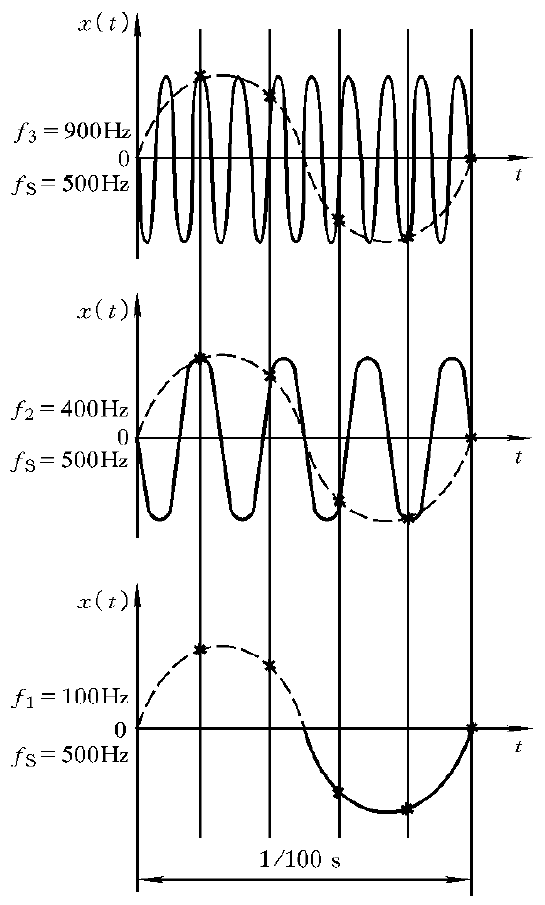
\includegraphics[width=7cm]{tex/1.png}
	\caption{$f_s < 2f_c$时.}
	\label{fig:31}
\end{figure}




\subsection{2}

通常对实验数据会在采集前设置前置滤波器,对采集到的数据, 通常在进行分析前也会采用数字滤波器,试分析这两个滤波器使 用的目的有何不同?如果$f_s<2f_c$,前置滤波器和后置滤波器的使 用区别在什么地方?

若$f_s<2f_c$,则采样得到的低频数据有可能是从高频数据来的。采集前设置前置滤波器,去掉$f>f_s/2$的部分,保证采样得到的低频部分是不受高频影响的。在进行分析前采用数字滤波器则是去掉不想研究的频段。前置滤波器对于有高频段数据来说是必要的,而分析前采用数字滤波器是为了分析数据而服务,可以自行选择。






% \nocite{*}

% \bibliographystyle{plain}

\phantomsection

\addcontentsline{toc}{section}{参考文献} %向目录中添加条目,以章的名义
\bibliography{homework}

\end{document}

